\documentclass[aspectratio=169]{beamer}
\usepackage{tikz}
\usepackage{graphicx}
\usepackage{listings}
\usepackage{xcolor}
\usepackage{hyperref}
\usepackage[spanish,es-noquoting]{babel}
\usepackage[round]{natbib}

\lstset{
  basicstyle=\ttfamily\small,
  keywordstyle=\color{blue},
  stringstyle=\color{red},
  commentstyle=\color{gray},
  showstringspaces=false
}

% Clean Theme Setup & Optimization
\usetheme{Warsaw}
\usecolortheme{default}
\usefonttheme{serif}

% Remove top headline bar and navigation clutter to maximize slide text space
\setbeamertemplate{headline}{}
\setbeamertemplate{navigation symbols}{}

% Slim, clean footline bar
\setbeamertemplate{footline}{
  \leavevmode%
  \hbox{%
    \begin{beamercolorbox}[wd=.333333\paperwidth,ht=2.25ex,dp=1ex,left]{author in head/foot}%
      \hspace*{2ex}\insertshortauthor
    \end{beamercolorbox}%
    \begin{beamercolorbox}[wd=.333333\paperwidth,ht=2.25ex,dp=1ex,center]{title in head/foot}%
      \insertshorttitle
    \end{beamercolorbox}%
    \begin{beamercolorbox}[wd=.333333\paperwidth,ht=2.25ex,dp=1ex,right]{date in head/foot}%
      \insertframenumber{} / \inserttotalframenumber\hspace*{2ex}
    \end{beamercolorbox}%
  }%
  \vskip0pt%
}

% Font size and list spacing optimizations to prevent text overflow
\setbeamertemplate{itemize/enumerate body begin}{\small}
\setbeamertemplate{itemize/enumerate subbody begin}{\footnotesize}
\setbeamertemplate{itemize/enumerate subsubbody begin}{\scriptsize}

\makeatletter
\g@addto@macro\itemize{%
  \setlength{\itemsep}{2pt}%
  \setlength{\parsep}{1pt}%
  \setlength{\topsep}{2pt}%
  \setlength{\partopsep}{0pt}%
}
\makeatother

\graphicspath{{../}{./}}
\setbeamertemplate{caption}[numbered]

% Title info
\title[ Escalando tu PromptLibrary]{ Escalando tu PromptLibrary}
\subtitle{ De los prompts iniciales a un sistema que crece contigo}
\author{Ricardo Reyes-Jimenez}
\institute{Universidad de La Sabana}
\date{\today}


% Background image for title slide
\usebackgroundtemplate{
  \tikz\node[opacity=0.3]{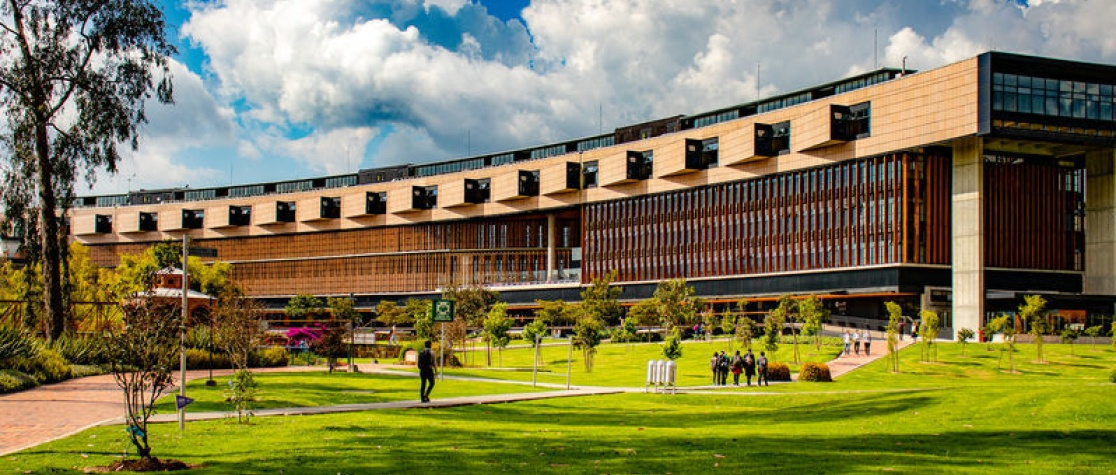
\includegraphics[width=\paperwidth,height=\paperheight]{Images/UniSabana.jpg}};
}


\begin{document}

% Title slide
\begin{frame}
  \titlepage
\end{frame}

% Reset background for normal slides
\usebackgroundtemplate{}


\begin{frame}[allowframebreaks,fragile]{Objetivos de la Sesión 2}

\begin{itemize}
  \item Dominar el arte del refinamiento de prompts (Troubleshooting).
  \item Aprender a construir ``Prompts Modulares'' o cadenas de instrucciones.
  \item Trazar la hoja de ruta tecnológica: Del Excel inicial a SharePoint.
  \item Entender la Gobernanza y el rol del Comité de Innovación/IA.
  \item Diseñar la política interna de incentivos para asegurar adopción.
\end{itemize}
\end{frame}

\begin{frame}[allowframebreaks,fragile]{Recapitulación: ¿Qué tenemos hasta ahora?}

\begin{itemize}
  \item Tenemos un archivo compartido (Excel/Word).
  \item Tenemos \textit{Blueprints} con variables (corchetes).
  \item Identificamos que el primer intento \textbf{casi siempre requiere ajustes}. La IA puede ser muy creativa cuando queremos precisión, o muy literal cuando queremos creatividad.
\end{itemize}
\end{frame}

\begin{frame}[allowframebreaks,fragile]{El ciclo de vida de un Prompt}

\begin{itemize}
  \item \textbf{Creación:} Se diseña el Blueprint base.
  \item \textbf{Prueba:} Se ejecuta con un caso real.
  \item \textbf{Falla (Feedback):} La IA hace algo no deseado (ej. inventa un dato, cambia el tono).
  \item \textbf{Refinamiento:} Se edita el Blueprint agregando restricciones.
  \item \textbf{Aprobación:} Se sube a la versión oficial de la biblioteca.
\end{itemize}
\end{frame}

\begin{frame}[allowframebreaks,fragile]{Refinamiento Individual: Iteración}

\begin{itemize}
  \item \textbf{El primer prompt nunca es el definitivo.}
  \item Si la IA se equivoca, la culpa rara vez es de la IA. Es ambigüedad en nuestras instrucciones.
  \item \textbf{Técnica del `\texttt{Few-Shot'':} Si las instrucciones no bastan, agrega al Blueprint un ejemplo de cómo quieres que se vea el resultado (un }`Shot'').
\end{itemize}
\end{frame}

\begin{frame}[allowframebreaks,fragile]{Caso Práctico de Refinamiento}

\begin{itemize}
  \item \textbf{Blueprint Original:} ``Resume este caso.'' (Produce 5 páginas de prosa densa).
  \item \textbf{Refinamiento 1 (Formato):} ``Resume este caso en 3 viñetas.''
  \item \textbf{Refinamiento 2 (Restricción):} ``Resume este caso en 3 viñetas. NO incluyas opiniones doctrinales, solo hechos probados.''
  \item \textbf{Refinamiento 3 (Rol):} ``Actúa como un juez laboral severo...''
\end{itemize}
\end{frame}

\begin{frame}[allowframebreaks,fragile]{El Feedback Loop: Cuando el prompt falla}

\begin{itemize}
  \item Si el modelo alucina: Faltó `\texttt{Anclaje'' (Grounding). Agrega la instrucción: \textit{}`Basate ÚNICAMENTE en el texto proporcionado. Si no encuentras la respuesta, di 'No hay información suficiente'''}.
  \item Si el modelo divaga: Falta enfoque. Acota la tarea. \textit{``Limítate a analizar la cláusula de terminación, ignora el resto del contrato.''}
\end{itemize}
\end{frame}

\begin{frame}[allowframebreaks,fragile]{Refinamiento Grupal: Inteligencia Colectiva}

\begin{itemize}
  \item Lo que le funciona al Abogado A en temas corporativos, puede fallarle al Abogado B en temas laborales.
  \item Compartir el \textit{Blueprint} con el equipo permite someterlo a ``Stress Testing'' con diferentes tipos de documentos y estilos de redacción.
  \item El consenso genera un Blueprint ``Gold Standard''.
\end{itemize}
\end{frame}

\begin{frame}[allowframebreaks,fragile]{El ``Prompt Modular'' (Encadenamiento)}

\begin{itemize}
  \item Las tareas jurídicas complejas no se resuelven con un solo super-prompt gigantesco, sino con una cadena de prompts pequeños (Pipeline).
  \item \textbf{Paso 1:} ``Extrae todas las fechas de este documento.''
  \item \textbf{Paso 2:} ``Con las fechas extraídas en el paso 1, construye una línea de tiempo cronológica.''
  \item \textbf{Paso 3:} ``Identifica si hay vacíos temporales de más de 6 meses en esa línea de tiempo.''
\end{itemize}
\end{frame}

\begin{frame}[allowframebreaks,fragile]{Integración en el Flujo de Trabajo}

\begin{itemize}
  \item Un Blueprint guardado en un Excel que nadie abre es inútil.
  \item Debemos integrar la PromptLibrary en las pantallas donde el abogado pasa el 90\% de su tiempo: Teams, Outlook, Word.
  \item Si está a más de 3 clics de distancia, la adopción caerá drásticamente.
\end{itemize}
\end{frame}

\begin{frame}[allowframebreaks,fragile]{Escalabilidad: Fase 1 (Personal)}

\begin{itemize}
  \item \textbf{``Mi bloc de notas'' (Notion, Evernote, Sticky Notes).}
  \item \textbf{Ventajas:} Rápido de crear, altamente personalizado, curva de aprendizaje cero.
  \item \textbf{Desventajas:} El conocimiento muere con el individuo. No hay control de calidad. No escala. Es la etapa inicial obligatoria.
\end{itemize}
\end{frame}

\begin{frame}[allowframebreaks,fragile]{Escalabilidad: Fase 2 (Compartida)}

\begin{itemize}
  \item \textbf{Excel en OneDrive / Canal de Teams.}
  \item \textbf{Ventajas:} Colaborativo, barato, permite ver qué están haciendo otros.
  \item \textbf{Desventajas:} Fricción para encontrar la información. Nadie audita si el prompt 23 es mejor que el 45. Peligro de desorden extremo (El síndrome de la carpeta ``Varios'').
\end{itemize}
\end{frame}

\begin{frame}[allowframebreaks,fragile]{Escalabilidad: Fase 3 (Institucional)}

\begin{itemize}
  \item \textbf{SharePoint / Intranet Custom / Herramientas Especializadas.}
  \item Repositorio oficial con buscador por palabras clave y sistema de etiquetas (Tags: \textit{\#Corporate, \#Litigation, \#DueDiligence}).
  \item Solo contiene `\texttt{Prompts Aprobados''. Es la }`Ley'' de la firma en uso de IA.
\end{itemize}
\end{frame}

\begin{frame}[allowframebreaks,fragile]{Gobernanza: El Comité de IA}

\begin{itemize}
  \item \textbf{¿Quién decide qué prompt entra a la versión oficial?}
  \item Se necesita un `\texttt{Líder de Innovación'' o un }`Comité de IA'' (socios + TI) encargado de validar y aprobar nuevos Blueprints.
  \item Este comité también revisa riesgos de privacidad antes de autorizar un flujo de trabajo.
\end{itemize}
\end{frame}

\begin{frame}[allowframebreaks,fragile]{Sostenibilidad: Auditoría de Modelos}

\begin{itemize}
  \item \textbf{La IA no es estática.} Los modelos reciben actualizaciones constantes (GPT-4 vs GPT-4o vs Claude 3.5).
  \item Un prompt que funcionaba perfecto hace 6 meses usando una técnica, hoy podría causar que la IA se confunda.
  \item \textbf{Regla de oro:} Auditar y re-probar los \textit{Blueprints} más críticos cada 3 a 6 meses.
\end{itemize}
\end{frame}

\begin{frame}[allowframebreaks,fragile]{Cultura y Adopción: El Reto Principal}

\begin{itemize}
  \item El mayor reto tecnológico no es el código, es la cultura humana.
  \item Si el Socio Director no usa, o peor aún, desconfía de la PromptLibrary, los abogados junior no la usarán.
  \item Hay que predicar con el ejemplo (Tone at the top).
\end{itemize}
\end{frame}

\begin{frame}[allowframebreaks,fragile]{Gamificación e Incentivos}

\begin{itemize}
  \item ¿Cómo motivamos a la firma a documentar?
  \item Premiar el esfuerzo: Reconocer públicamente al abogado que aportó el \textit{Blueprint} que más horas ahorró en el mes.
  \item Algunos despachos incluyen el ``Uso e innovación en IA'' como KPI para los bonos anuales de los asociados.
\end{itemize}
\end{frame}

\begin{frame}[allowframebreaks,fragile]{Taller Práctico Final: Diseñando tu Gobernanza}

\textbf{Dinámica en Grupos (20 Minutos):}
\begin{itemize}
  \item Redacten un borrador rápido (flujograma) del proceso de aprobación de su firma. Desde que el practicante crea un prompt hasta que llega a SharePoint.
  \item Definan 2 métricas de éxito (KPIs) para medir si la biblioteca realmente sirve.
  \item Propongan 1 incentivo para que los abogados contribuyan mensualmente.
\end{itemize}
\end{frame}

\begin{frame}[allowframebreaks,fragile]{Presentación de Propuestas}

\textbf{Plenaria (15 Minutos):}
\begin{itemize}
  \item Compartamos las estrategias de gobernanza.
  \item ¿Qué obstáculos reales ven en sus oficinas para implementar esto el lunes a las 8:00 AM?
  \item ¿Cómo podemos sortear esos obstáculos?
\end{itemize}
\end{frame}

\begin{frame}[allowframebreaks,fragile]{Cierre del Módulo 3}

\begin{itemize}
  \item La IA Generativa democratizó la programación. Escribir prompts es programar en español.
  \item Su PromptLibrary es ahora su código fuente. Trátenlo con el mismo cuidado que a su base de precedentes legales.
  \item ¡Felicitaciones por construir las bases tecnológicas de la firma del futuro!
\end{itemize}
\end{frame}




\end{document}